\documentclass{article}

\usepackage[a4paper, total={6in, 10in}]{geometry}
\usepackage[T2A]{fontenc}
\usepackage[utf8x]{inputenc}
\usepackage[english,russian]{babel}
\usepackage{graphicx}
\usepackage{float}
\usepackage{wrapfig}

\begin{document}
\begin{titlepage}
    \begin{center}
        \vspace*{5cm}

        \LARGE
        \textbf{Метрический алгоритм классификации kNN}
    
        \vspace{0.5cm}
 
        \textbf{Сорокин Олег, 317}
 
        \vfill
             
        \vspace{0.8cm}
      
        \normalsize
        каф. ММП, ВМК МГУ\\
        14.10.2022
             
    \end{center}
 \end{titlepage}

\newpage
\tableofcontents{}
\newpage

\section{Введение}
    Алгоритм KNN - метрический алгоритм, применяющийся в задачах
    классификации или регрессии. Является достаточно
    простым и популярным (в том числе и в промышленности).

    Далее будем рассматривать только модель классификации на основе KNN.
    Пользуясь собственной реализацией на Python с использованием библиотеки numpy и алгоритмами sklearn на примере данных из MNIST:
    \begin{itemize}
        \item сравним эффективность различных алгоритмов поиска в условиях большой размерности
        признакового пространства;
        \item рассмотрим проблемы роста временных затрат с ростом числа данных
        или их размерности;
        \item предложим возможные методы подбора гиперпараметров с целью увеличения качества модели.
        Ориентиром качества выберем модели классификации, упоминания о которых
        есть на Kaggle, и с помощью которых решалась задача с такими же
        данными;
        \item рассмотрим иные методы увеличения точности классификации.
    \end{itemize}

\section{Список экспериментов}
    \subsection{Сравнение по времени алгоритмов поиска ближайших соседей}
        \subsubsection{Дизайн эксперимента}
            Выборка содержит 70тыс. grayscale-изображений цифр от 0 до 9 размера 28x28 пикселей.
            Разобьём её на тренировочную (первые 60тыс.) и тестовую (остальные 10тыс.).
            Будем искать $k=5$ ближайших соседей из второй выборки для каждого объекта первой выборки, сравнивая время, затрачиваемое каждым алгоритмом.
            Предварительно получим данные разных размерностей, отбросив часть признаков для объектов обеих выборок следующим образом:
            \begin{itemize}
                \item Каждое из изображений по строкам вытягиваем в вектор длины 28*28 = 784
                \item От каждого из векторов $(x_1, x_2, ..., x_{784})$ выберем подвекторы $(x_1, x_2, ..., x_s)$, где $s \in \{10, 20, 100\}$
            \end{itemize}

            Измерения будем производить, подавая на вход часть описание единственного объекта тестовой выборки.
            Зафиксируем гиперпараметры модели: метрика - евклидова, $k=5$ - выбрано ранее.
            Сравним время выполнения поставленной задачи для алгоритмов поиска: brute-перебор, kd-tree, ball-tree из библиотеки sklearn, а также для реализации my\_own на основе построения матрицы попарных расстояний.
        \subsubsection{Результаты}
            Средние значения времени по каждой из рассматриваемых размерностей приведены в таблице:
            \begin{center}
                \begin{tabular}{ c | c | c | c  }
                    Алгоритм & $t_{cp}, dim=10$ & $t_{cp}, dim=20$ & $t_{cp}, dim=100$ \\
                    \hline
                    my\_own & 0.00205 & 0.0034 & 0.01246 \\
                    \hline
                    brute & 0.00124 & 0.00144 & 0.00486 \\
                    \hline
                    kd-tree & 0.00133 & 0.00208 & 0.00742 \\
                    \hline
                    ball-tree & 0.00119 & 0.00165 & 0.00637 \\
                \end{tabular}
                \end{center}
        \subsubsection{Выводы}
                В данной задаче лучше всего себя проявил bruteforce алгоритм.
                Его сложность, согласно документации, составляет $O(DN^2)$, где
                $D$ - размерность данных, $N$ - число элементов.
                Для сравнения, сложность, например, kd-tree составляет $O(D*N*logN)$.
                Из полученных результатов следует, что константа О большого в общем случае может быть велика.
                Значит, для достаточно малого числа элементов и достаточно малых размерностей эффективнее использовать bruteforce.

                Стоит, однако, заметить, что результаты получены при значительном ограничении $N=1$. С ростом $N$ kd-tree начинает проявлять свою эффективность.
    \subsection{Влияние гиперпараметров модели на её точность}
        \subsubsection{Дизайн эксперимента}
                Исследуем, как метрика и число ближайших соседей влияют на точность классификации рассматриваемых данных из MNIST.
                Каждой из двух исследуемых метрик (евклидова и косинусная) поставим в соответствие классификатор.
                Зафиксируем стратегию поиска классификаторов и схему использования весов. Например, возьмём алгоритм my\_own с равномерными весами для каждого соседа.
                Далее проверим все $k = 1, ..., 10, 250$ для классификатора с евклидовой метрикой и для классификатора с косинусным расстоянием.
                При этом будем использовать кросс-валидацию с тремя фолдами. Усреднив результаты по фолдам, получим средние точности для каждого $k$.
                Далее сделаем выводы о том, при каких $k$ показал лучшую точность каждый из классификаторов.
        \subsubsection{Результаты}
                Результаты эксперимента отражены на рисунках 1-3:
                \begin{figure}[H]
                    \centering
                    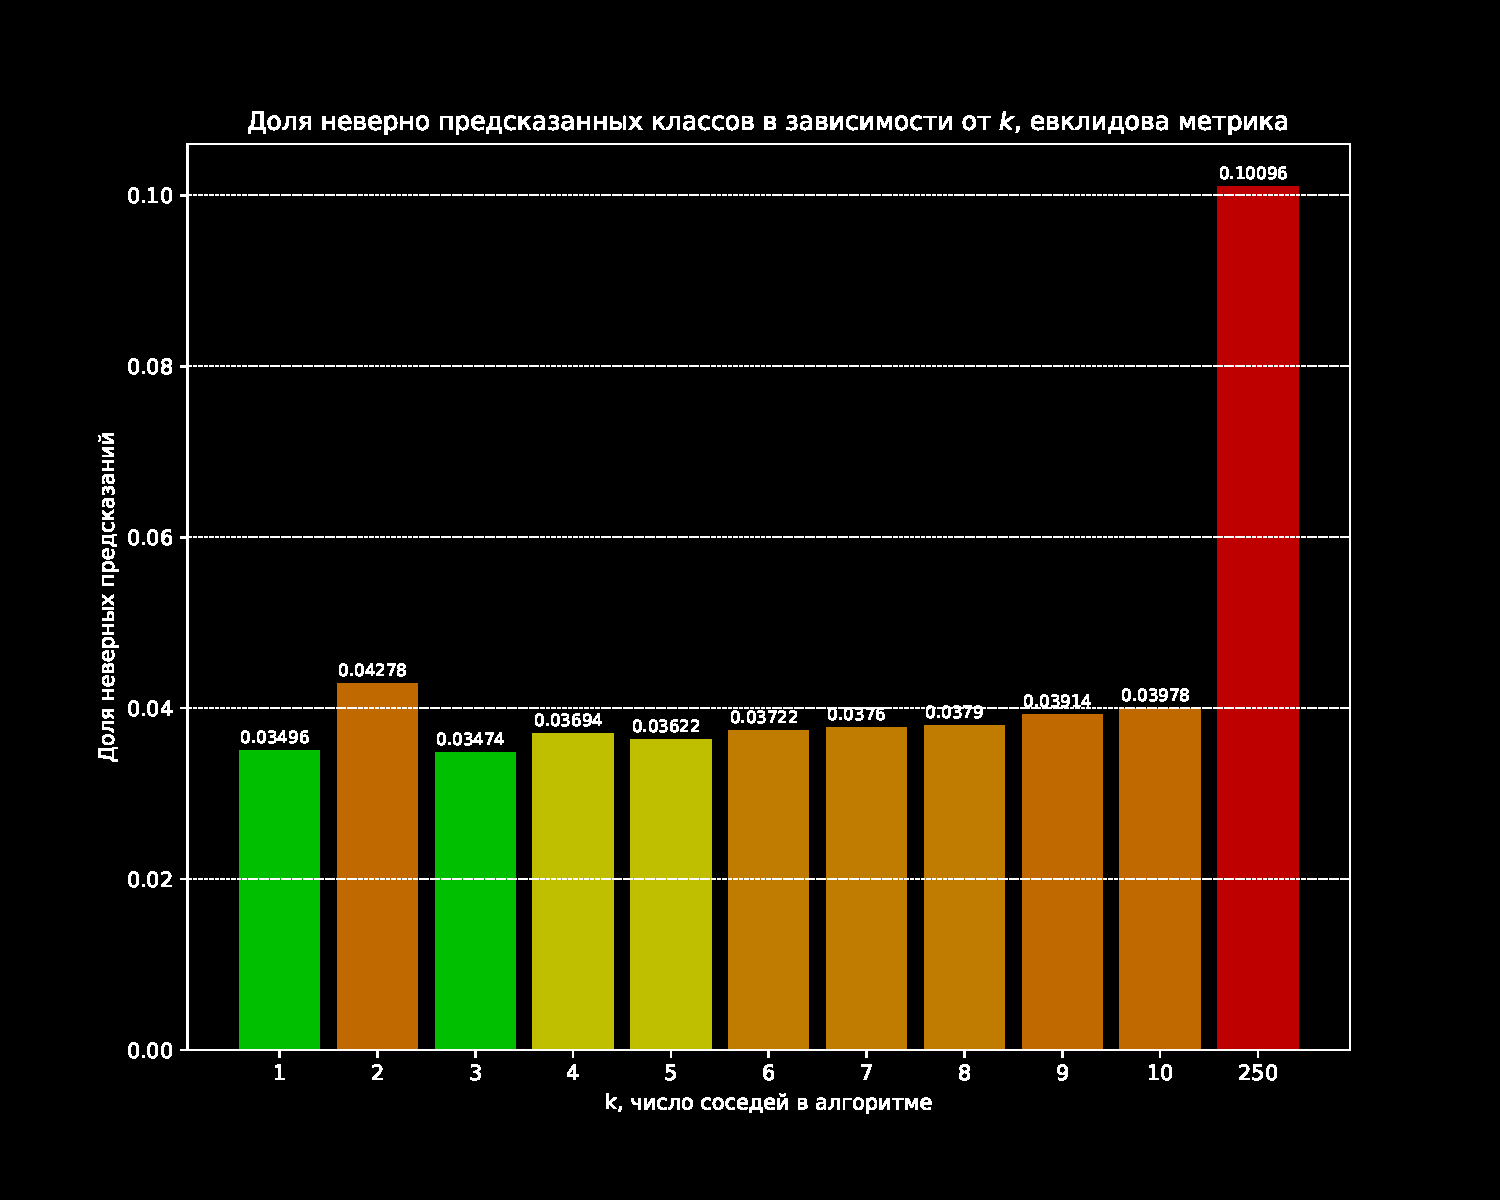
\includegraphics[width=0.8\linewidth]{./pictures/Euclidean.pdf}
                    \caption{Результат для евклидовой метрики}
                    \label{fig:mpr}
                \end{figure}

                \begin{figure}[H]
                    \centering
                    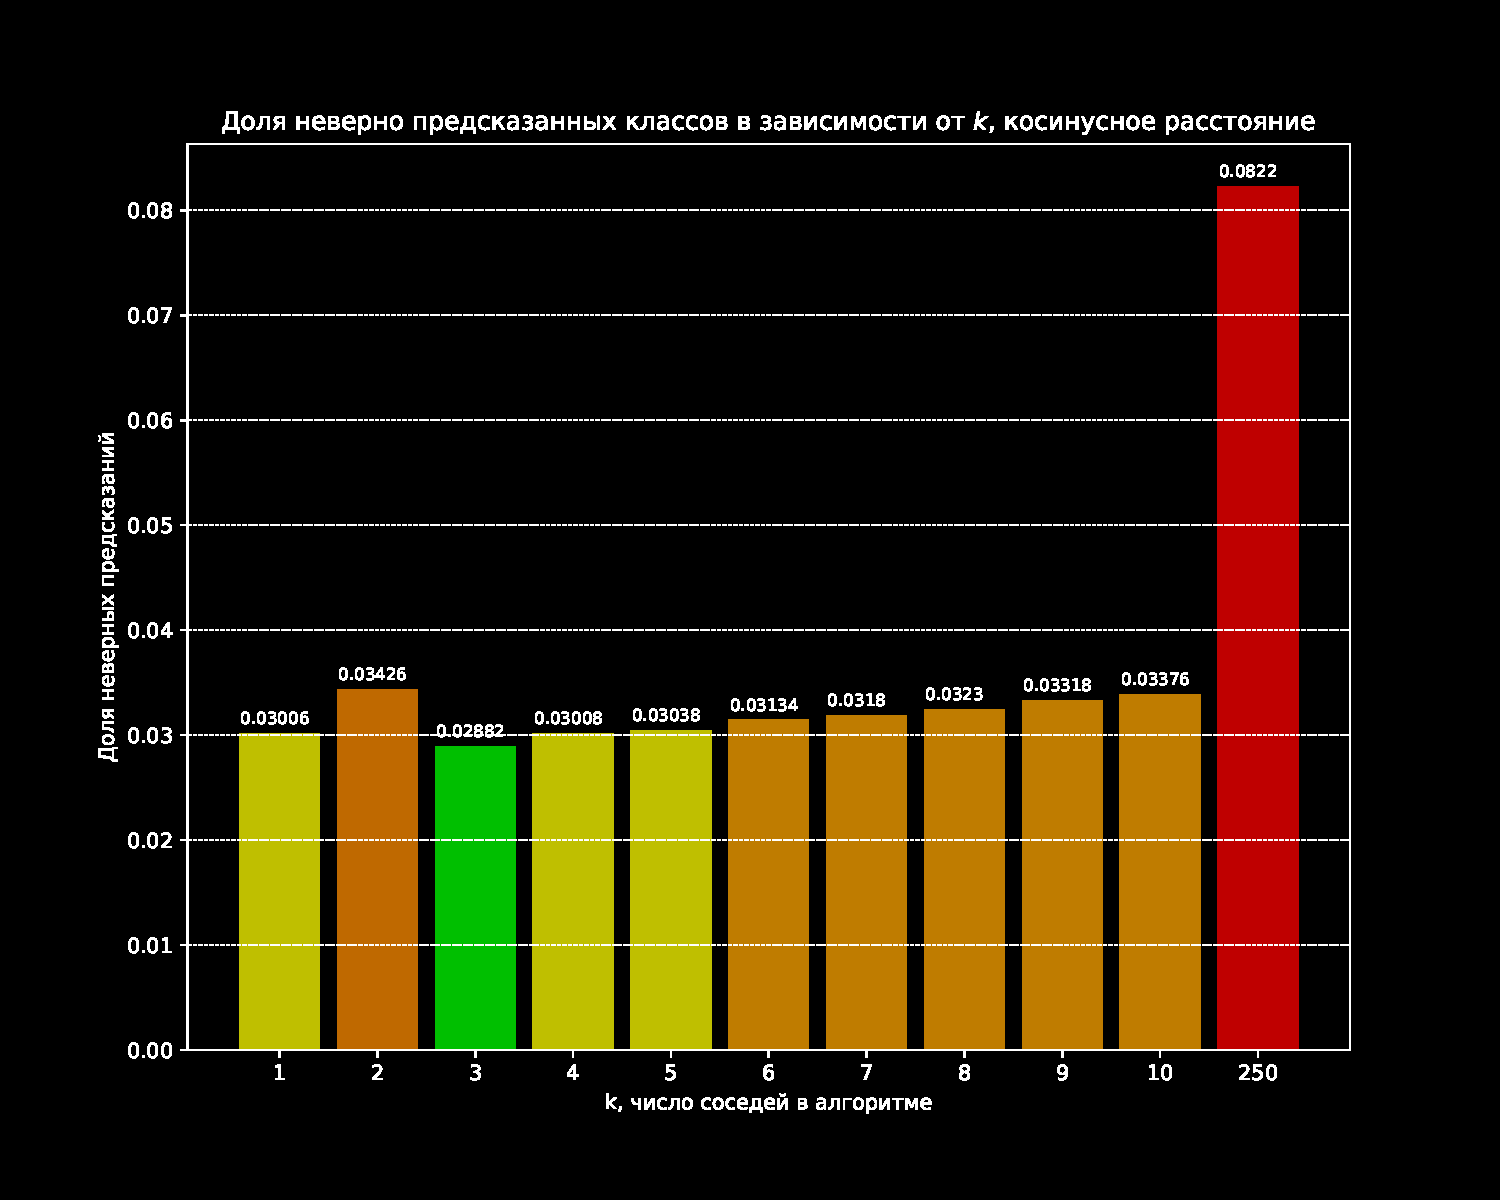
\includegraphics[width=0.8\linewidth]{./pictures/Cosine.pdf}
                    \caption{Результат для косинусного расстояния}
                    \label{fig:mpr}
                \end{figure}

                \begin{figure}[H]
                    \centering
                    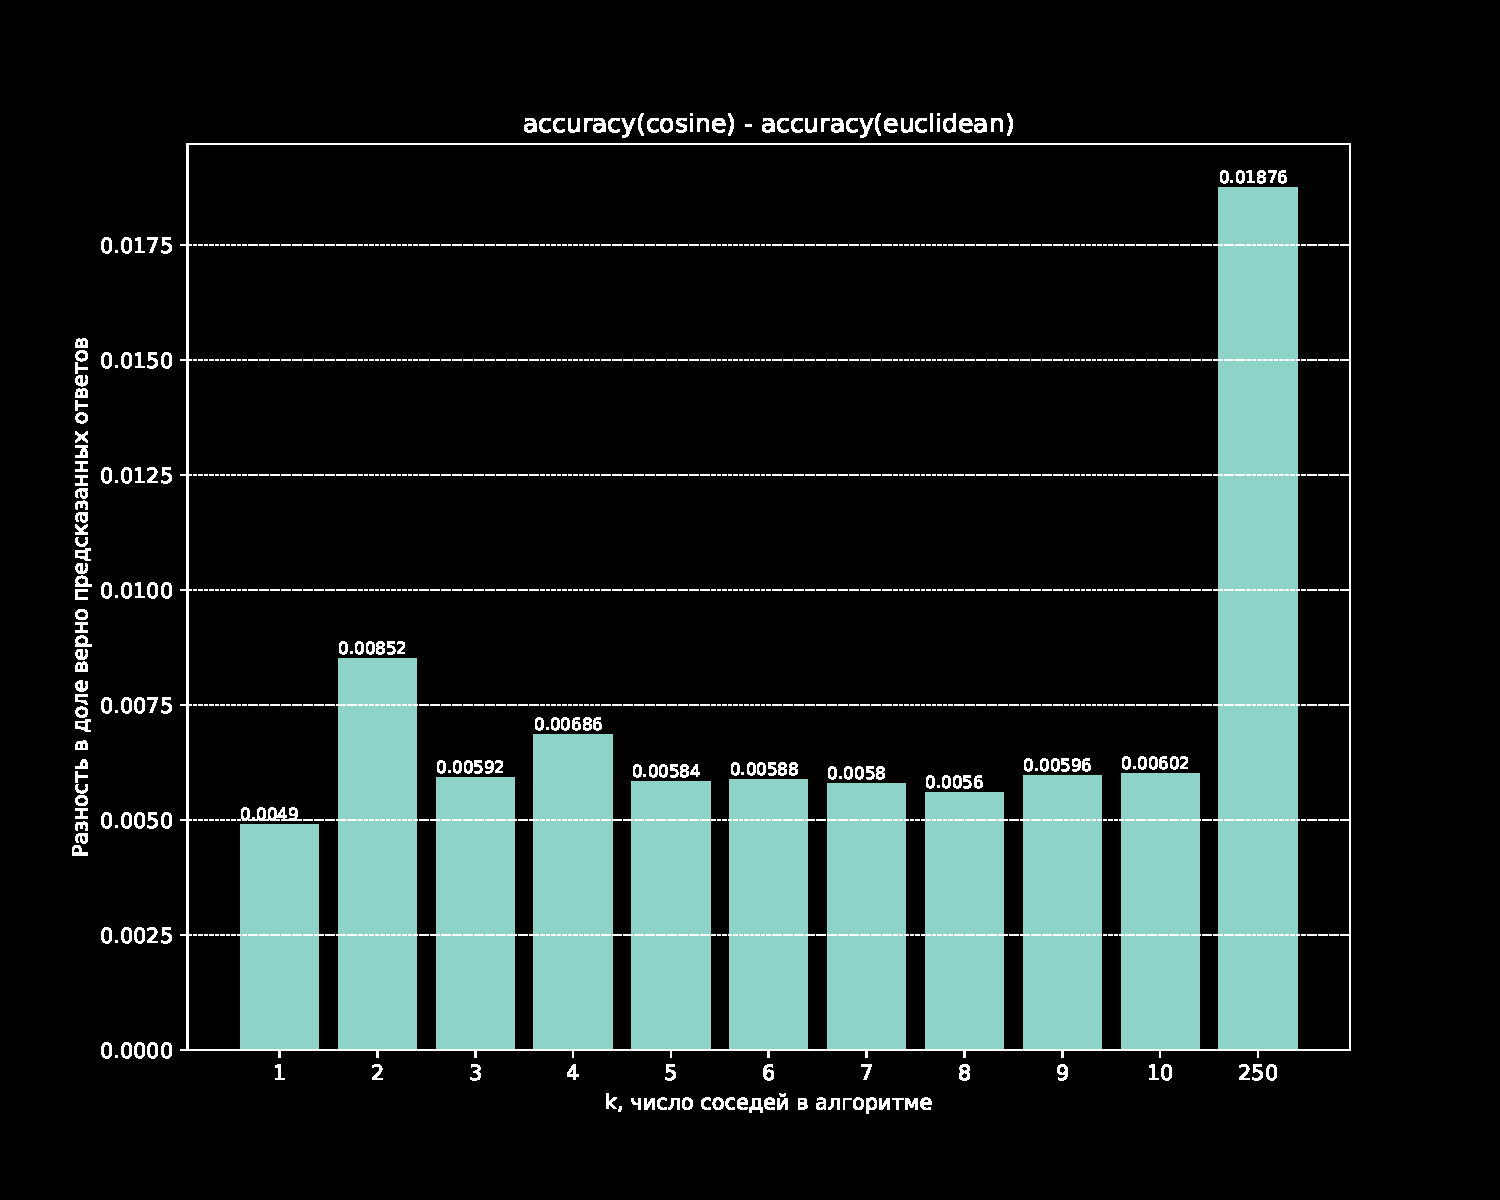
\includegraphics[width=0.8\linewidth]{./pictures/Delta.pdf}
                    \caption{Разностное сравнение двух метрик}
        \subsubsection{Выводы}
                Наибольшая точность достигается при некотором промежуточном значении $k$, то есть $k > 1$ и $k << |X_{train}|$.
                Действительно, $k=1$ соответствует самой сложной модели в том смысле, что происходит запоминание позиций, что ведёт к переобучению модели.
                И напротив, большие значения $k$ означают, что модель переупрощена, то есть неспособна выискивать паттерны в виде групп ближайших соседей одного класса.
                Частично эта проблема может быть решена с помощью весовых схем (см. след. эксперимент).
                На графиках можно видеть, что некоторые значения могут работать лучше соседних.
                Объяснение этому состоит в том, что в выборке в кластерах объектов могут присутствовать выбросы.
                При малых значениях $k$ модель может обнаружить только эти выбросы и ошибиться, а при больших - обнаружить объекты других классов за пределами кластера, что тоже приведёт к ошибочной классификации.

                На рис. 3 можно видеть, что при всех значениях $k$ лучше себя показало косинусное расстояние. Возможные объяснения:
                \begin{itemize}
                    \item Евклидова метрика подвержена проклятию высокой размерности (784 признака).
                    \item В многомерном пространстве для однозначного определения точки
                    нужно выбрать совокупность углов, откладываемых от осей и длину вектора.
                    Длина вектора при фиксированных углах в рассматриваемой задаче соответствует яркости изображения,
                    при этом при изменении длины вектора класс соответствующего объекта не меняется.
                    Косинусное расстояние, в отличие от евклидовой метрики, игнорирует монотонные перемены
                    в яркости изображения, а некоторые изображения из датасета действительно могут отличаться
                    лишь своей интенсивностью (см. раздел 4.1, аппендикс).
                \end{itemize}
    \subsection{Влияние наличия весов, зависящих от расстояний, на точность предсказаний}
        \subsubsection{Дизайн эксперимента}
                Проверим, увеличится ли точность при замене единичных весов на убывающие от расстояния.
                Зафиксируем некоторую конфигурацию модели, например, my\_own с косинусным расстоянием.
                Для $k = 1, ..., 10, 250$ сравним средние точности по трём фолдам для алгоритма без весов и для алгоритма, где вес $i$-го соседа объекта $x$ определяется как
                $$W(i, x) = \frac{1}{\rho(x, x^{(i)}) + \epsilon}, \epsilon = 10^{-5}$$
        \subsubsection{Результаты}
                Результат сравнения точностей представлен на графике:
                \begin{figure}[H]
                    \centering
                    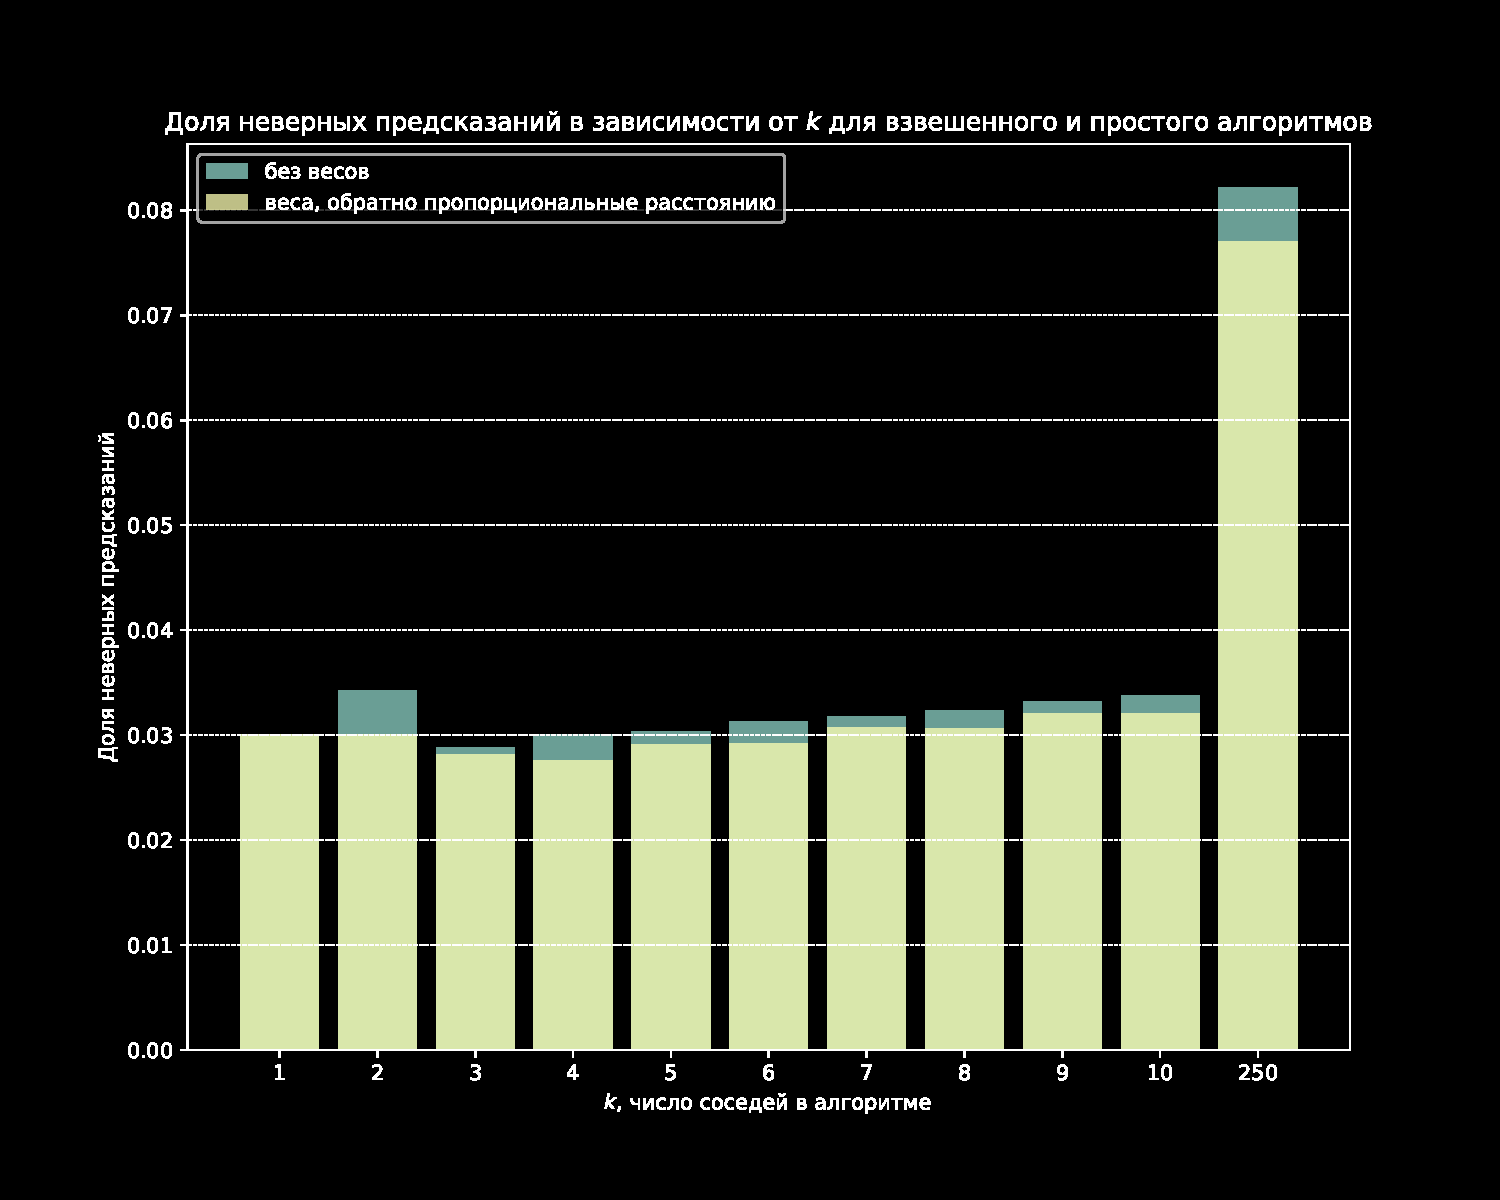
\includegraphics[width=0.8\linewidth]{./pictures/Weights.pdf}
                    \caption{Результат сравнения весовых схем KNN}
                    \label{fig:mpr}
                \end{figure}

        \subsubsection{Выводы}
                Наличие весов, заданных указанным способом, повышает точность классификации.

        \subsection{Анализ множества ошибочных предсказаний лучшего алгоритма}
            \subsubsection{Дизайн эксперимента}
                Из предыдущих экспериментов следует, что лучшим набором параметров в смысле точности является весовой алгоритм с косинусным расстоянием $k=4$.
                В качестве алгоритма поиска выберем bruteforce.

                Определим тренировочную и тестовую выборки как в эксперименте 1.
                Подсчитаем точность алгоритма на тестовой выборке, сравним с точностью по кросс-валидации. Выполним анализ ошибок на объектах тестовой выборки.
            \subsubsection{Результаты}
                На тренировочной выборке точность достигла 1.0, на тестовой выборке -- 0.9752.
                При разбиении по кросс-валидации (с тремя фолдами) исходной выборки для этих же параметров получим точности (0.97366053, 0.97174057, 0.97131885).


                Матрица ошибок имеет вид, указанный на рис. 5.
                \begin{figure}[h]
                    \centering
                    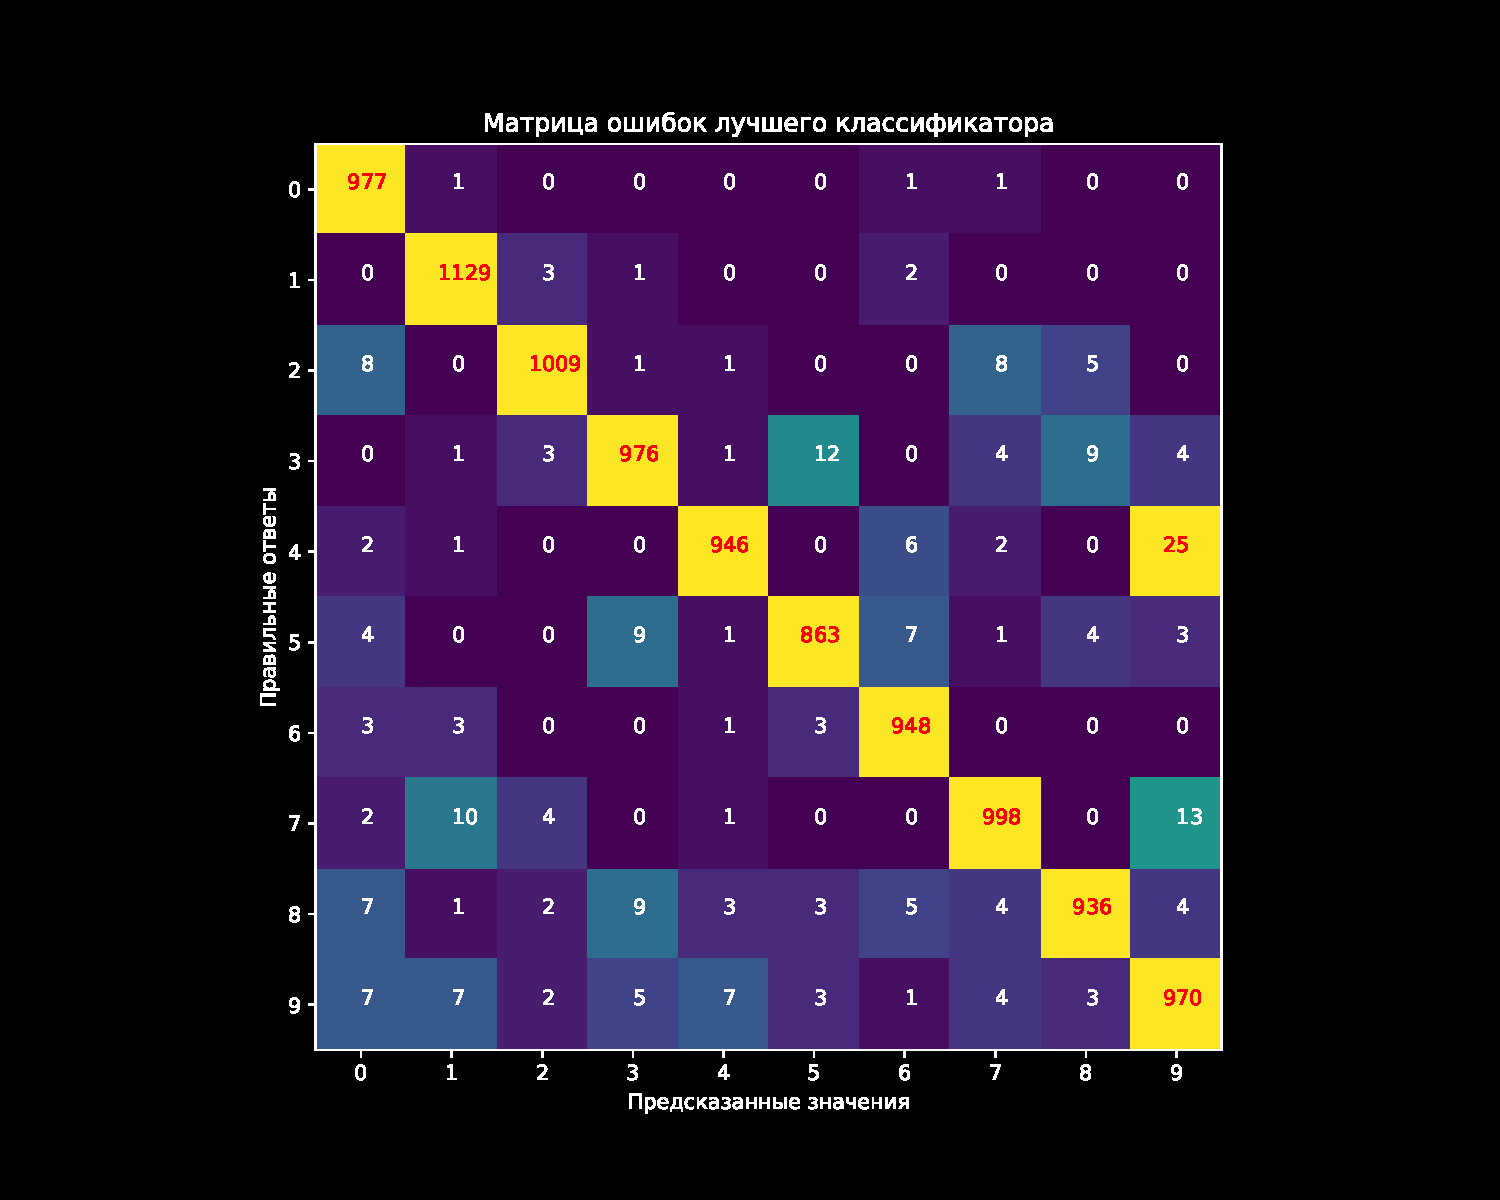
\includegraphics[width=0.8\linewidth]{./pictures/Confusion.pdf}
                    \caption{Матрица ошибок лучшего классификатора}
                    \label{fig:mpr}
                \end{figure}
            \subsubsection{Выводы}
                Лучший алгоритм на тестовой выборке показал примерно ту же точность, что и на кросс-валидации.
                Практически все современные алгоритмы показывают более высокие результаты (а у топовых алгоритмов точность на MNIST достигает порядка 0.99).

                Анализируя матрицу ошибок, можно сказать следующее:
                \begin{itemize}
                    \item Больше всего ошибок суммарно допущено при распознавании цифры 9 (39 ошибок).
                    \item Самая частая ошибка классификатора - отклик 9 на объекте класса 4 (25 ошибок).
                \end{itemize}

                На рис. 6 приведены примеры изображений, распознанных неверно.
                Среди их особенностей можно выделить нетипичность написания отдельных элементов цифры (некоторые и вовсе не дописаны).
                И, как можно видеть из примеров, это зачастую делает цифры плохо различимыми.
                \begin{figure}[H]
                    \centering
                    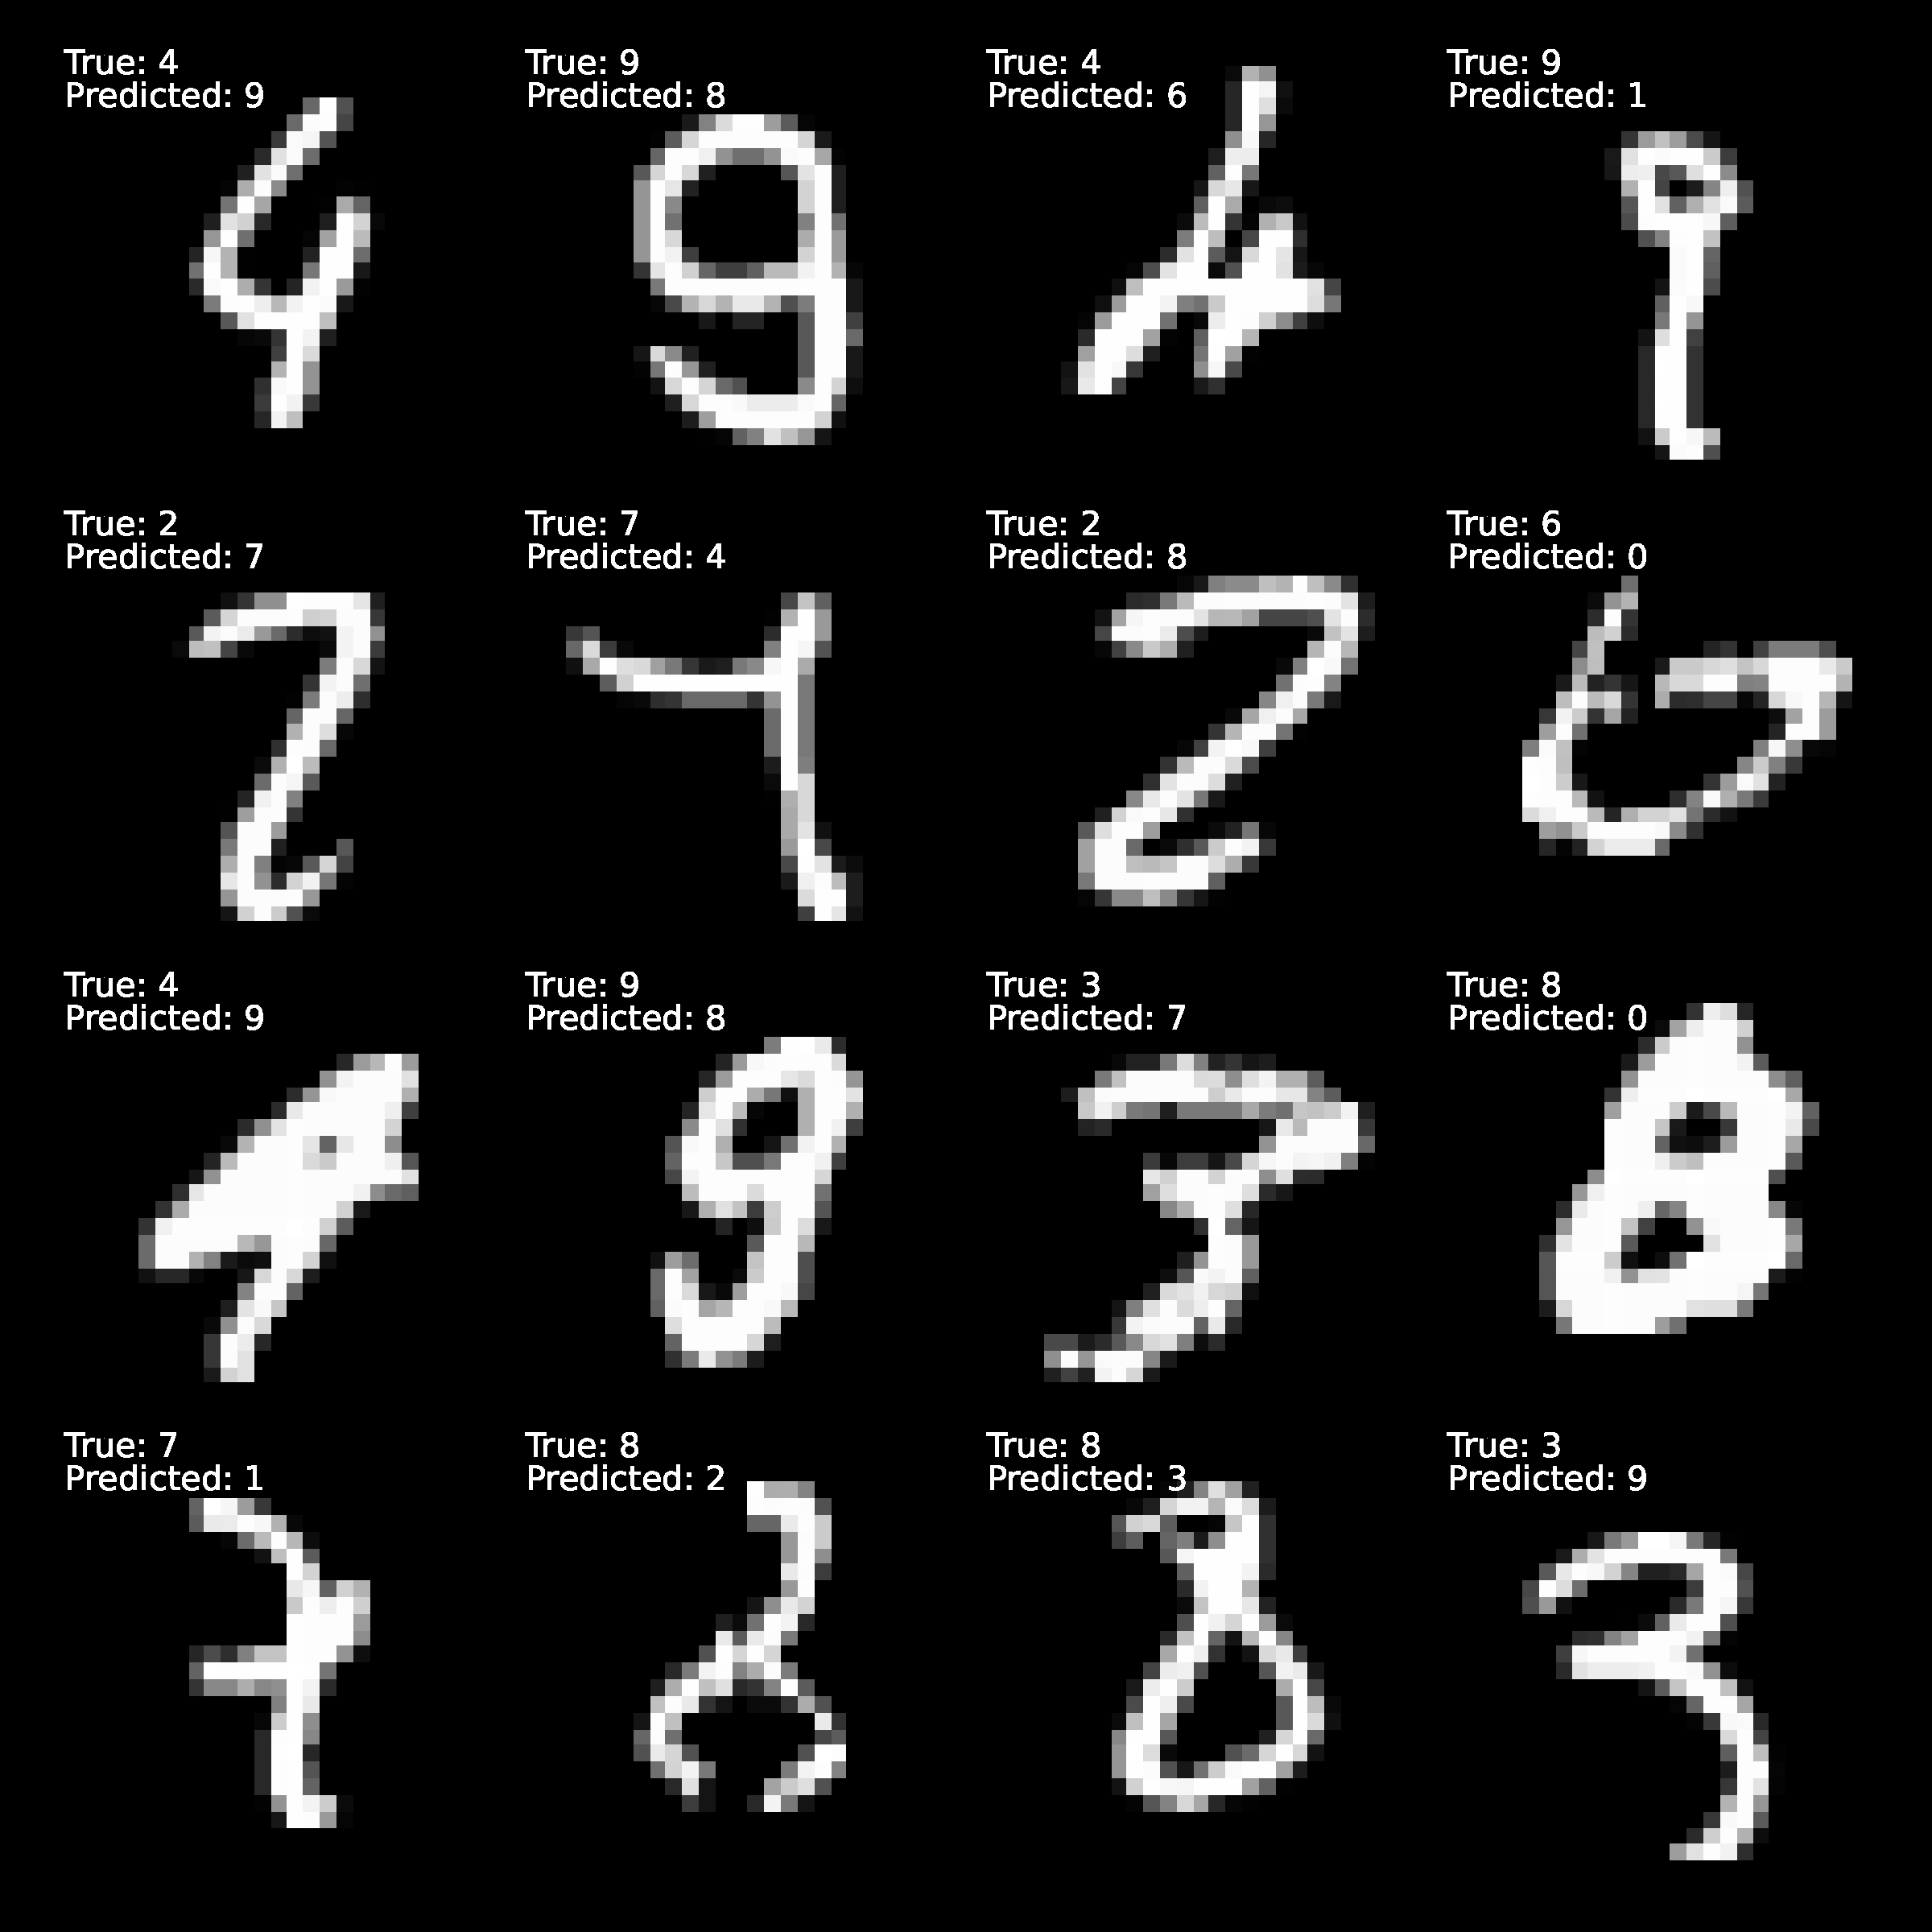
\includegraphics[width=0.8\linewidth]{./pictures/WrongExamples.pdf}
                    \caption{Примеры неверно классифицированных изображений}
                    \label{fig:mpr}
                \end{figure}

        \subsection{Влияние расширения выборки путём аугментации на точность предсказаний}
            \subsubsection{Дизайн эксперимента}
                Будем рассматривать следующие виды аугментации:
                \begin{enumerate}
                    \item[1)] Случайный поворот в обоих направлениях на 5, 10, 15 градусов.
                    \item[2)] Смещение на 1, 2, 3 пикселя по обеим осям.
                    \item[3)] Гауссовский фильтр с ядром 15, дисерсиями 0.5, 1.0, 1.5.
                    \item[4)] Морфологические преобразования: эрозия, дилатация, открытие, закрытие с ядром 2.
                \end{enumerate}

                Зафиксируем модель, описанную в предыдущем эксперименте.
                Реализуем жадный алгоритм поиска приводящих к увеличению точности преобразований над списом из $n$ преобразований:
                \begin{enumerate}
                    \item[0.] Преобразования к тренировочной выборке не применены, считаем точность модели.
                    \item[1.] Перебираем все параметры первого преобразования, выбираем наилучшее. Если качество ухудшилось по сравнению с предыдущей итерацией, переходим к следующей итерации с исходной выборкой, иначе - с преобразованной.
                    \item[$2...n)$.] Аналогично шагу 1.
                \end{enumerate}
                На шаге $n$ мы находим оптимальную комбинацию преобразований.

                Рост выборки - экспоненциальный, поэтому аугментировать на каждой итерации будем 20000 объектов.
            \subsubsection{Результаты}
                Изначальная точность -- 0.9752. В результате работы алгоритма были последовательно отобраны преобразования:
                \begin{itemize}
                    \item Поднятие точности до 0.978 поворотами на 10 градусов.
                    \item Поднятие точности до 0.9787 сдвигами на пиксель.
                    \item Поднятие точности до 0.9791 применением гауссовского фильтра с дисперсией 1.5.
                    \item Поднятие точности до 0.9797 применением открытия с ядром 2.
                \end{itemize}
                
            \subsubsection{Выводы}
                В разделе 4.2 (аппендикс) приведены 4 матрицы, каждая из которой есть разница новой и старой матриц ошибок (до и после аугментации). Используем их для отслеживания динамики ошибок в различных случаях.

                Поворот изображений наиболее поднял точность распознавания 3 и 9, а именно уменьшился процент предсказания вместо них 5 и 3 соответственно. Кроме того, лучше распознаётся 7 (не путается с единицей).

                Сдвиг незначительно увеличил процент распознавания 8 и 9.

                В исходном датасете находилось много недописанных цифр 8, гауссовский фильтр частично исправил эту ситуацию, уменьшив процент неверных предсказаний восьмёрок. Однако в связи с наложением шума на похожие изображения возникли ошибки с парами 3-5, 9-7, поэтому изменение точности не очень велико.

                Морфологические операции незначительно повлияли на некоторые ошибки, возникшие при аугментации с помощью фильтра Гаусса.

    \subsection{Влияние расширения тестовой выборки аналогичной аугментацией на точность}
        \subsubsection{Дизайн эксперимента}
            Обучим алгоритм на оригинальной подвыборке из 60000 элементов. Подобно предыдущему эксперименту будем применять жадный алгоритм, но аугментировать в этот раз будем тестовую выборку.
            Сделаем выводы о динамике ошибок, построив соответствующие матрицы.
        \subsubsection{Результаты}
            В результате работы жадного алогоритма нашлось только одно преобразование тестовой выборки, повышающее точность - гауссовский фильтр с дисперсией 0.5.
            Соответствующая матрица приведена на рис. 7.
            \begin{figure}[h]
                \centering
                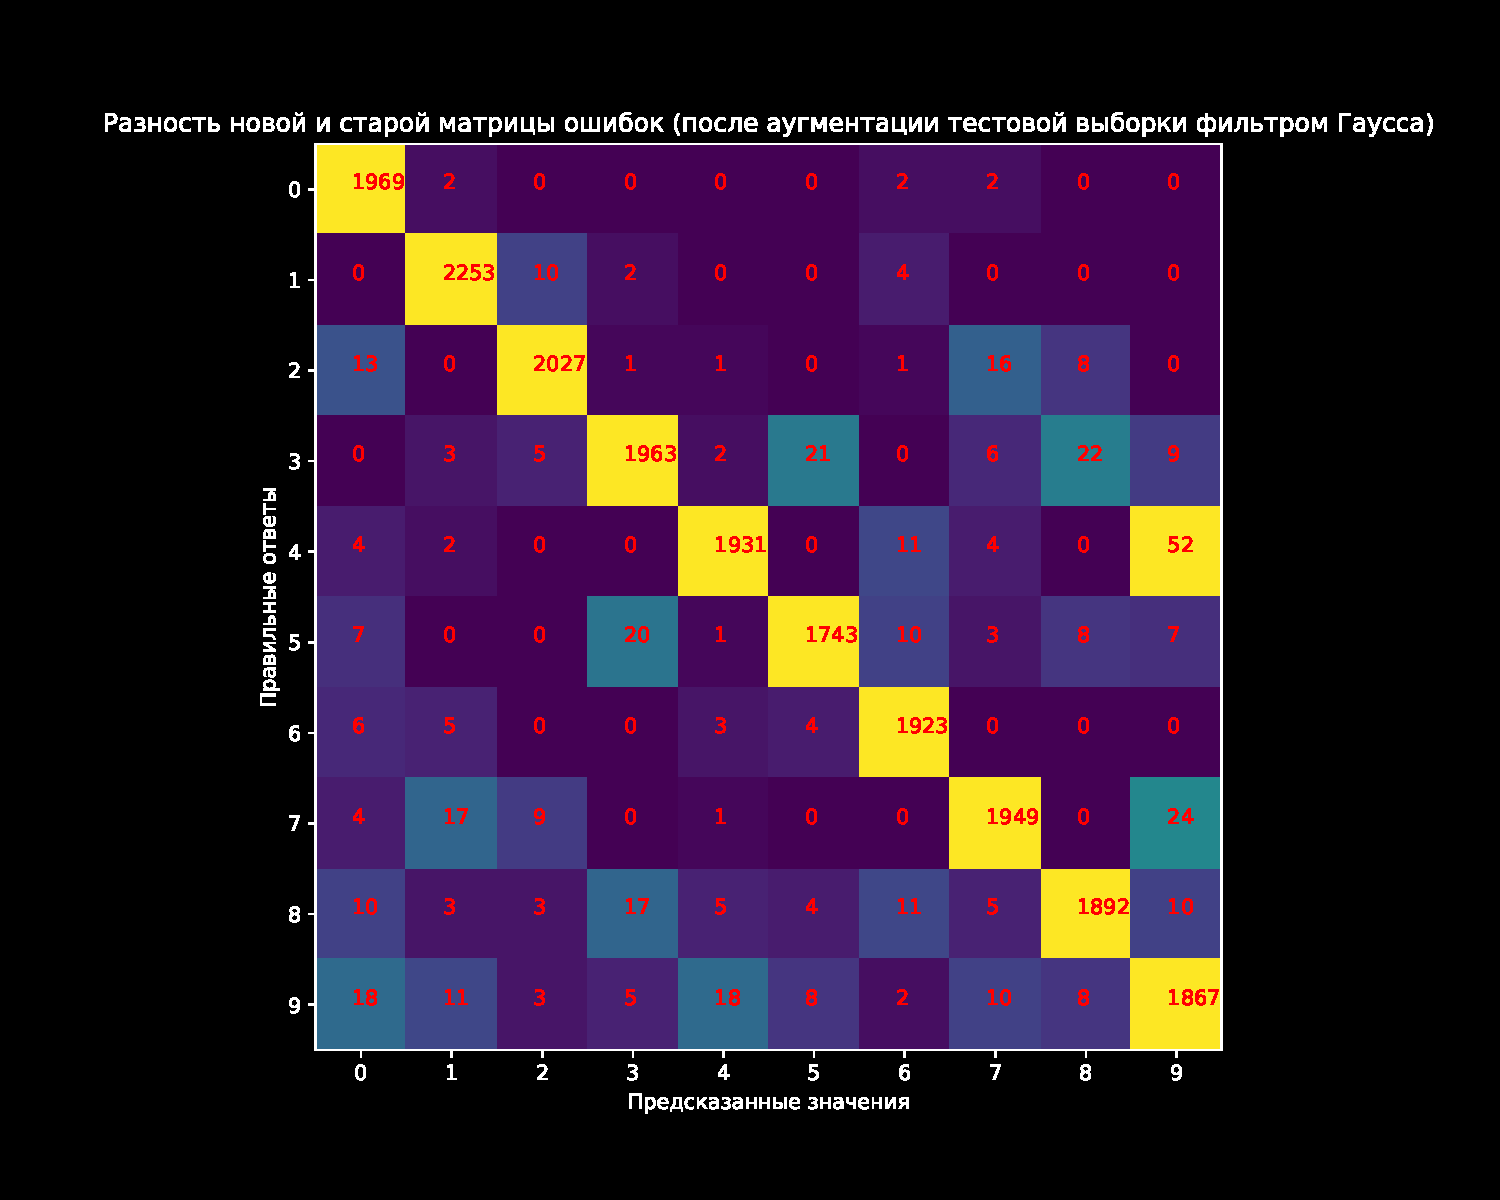
\includegraphics[width=0.8\linewidth]{./pictures/ConfusionDifferenceBlur6.pdf}
                \caption{Матрица ошибок после аугментации тестовой выборки фильтром Гаусса}
                \label{fig:mpr}
            \end{figure}

        \subsubsection{Выводы}
            Метод, описанный в эксперименте 5, привёл к значительному увеличению точности.
            Аугментирование тестовой выборки практически не повлияло на точность.
            Возможно, её изменение обусловлено тем, что фильтр Гаусса сильнее всего повлиял на объекты, которые модель часто классифицировала неверно.

\section{Выводы}
            Из существующих алгоритмов поиска ближайших соседей нельзя выбрать универсальный.
            Как было показано, даже bruteforce алгоритм может быть эффективен в задачах высокой размерности при малых данных,
            тогда как деревья могут проигрывать ему в этой ситуации.

            Не существует и единого подхода в выборе гиперпараметров: в задачах низких размерностей, рассматриваемых на Kaggle,
            высокие результаты показывает евклидова метрика. В рассматриваемой здесь задаче по указанным ранее причинам
            косинусное расстояние приводит к большему увеличению точности модели.

            Однозначно положительный эффект на работу модели оказывает аугментация обучающей выборки.
            В условиях недостаточного количества данных (а при высокой размерности признакового пространства выборка не содержит достаточно информации о каждом единичном объекте) она является надёжным методом повышения точности.

\section{Аппендикс}
    \subsection{Пояснение к сравнению качества работы при различных метриках}
    Рассмотрим следующие изображения (второе инвертировано для лучшей различимости):

        \begin{figure}[H]
        \centering
        
\includegraphics[width=0.8\linewidth]{./pictures/EuclideanVSCosine.pdf}
        \caption{Иллюстрация к примеру о сравнении метрик}
        \label{fig:mpr}
        \end{figure}

    Пронумеруем их слева направо от 1 до 3. Матрица $M$ попарных евклидовых расстояний имеет вид:
        \begin{center}
            \begin{tabular}{ c | c  c  c  }
                & 1 & 2 & 3 \\
                \hline
                1 & 0 & 3160 & 3139 \\
                2 & 3160 & 0 & 2225 \\
                3 & 3139 & 2225 & 0 \\
            \end{tabular}
            \end{center}
            Для попарных косинусных расстояний имеем:
            \begin{center}
                \begin{tabular}{ c | c  c  c  }
                    & 1 & 2 & 3 \\
                    \hline
                    1 & 0.0 & 0.14 & 0.59 \\
                    2 & 0.14 & 0.0 & 0.62 \\
                    3 & 0.59 & 0.62 & 0.0 \\
                \end{tabular}
                \end{center}
            Объекты 1 и 2 следует отнести к одному классу, 1 и 3 - к разным.
            Однако при этом евклидово расстояние между объектами 1 и 2 больше расстояния между объектами 1 и 3, что может привести к ошибке классификации.
            Косинусное расстояние, как было описано ранее, менее чувствительно к смене
            яркости.

    \subsection{Разности матриц из эксперимента 5}
        \begin{figure}[H]
            \centering
            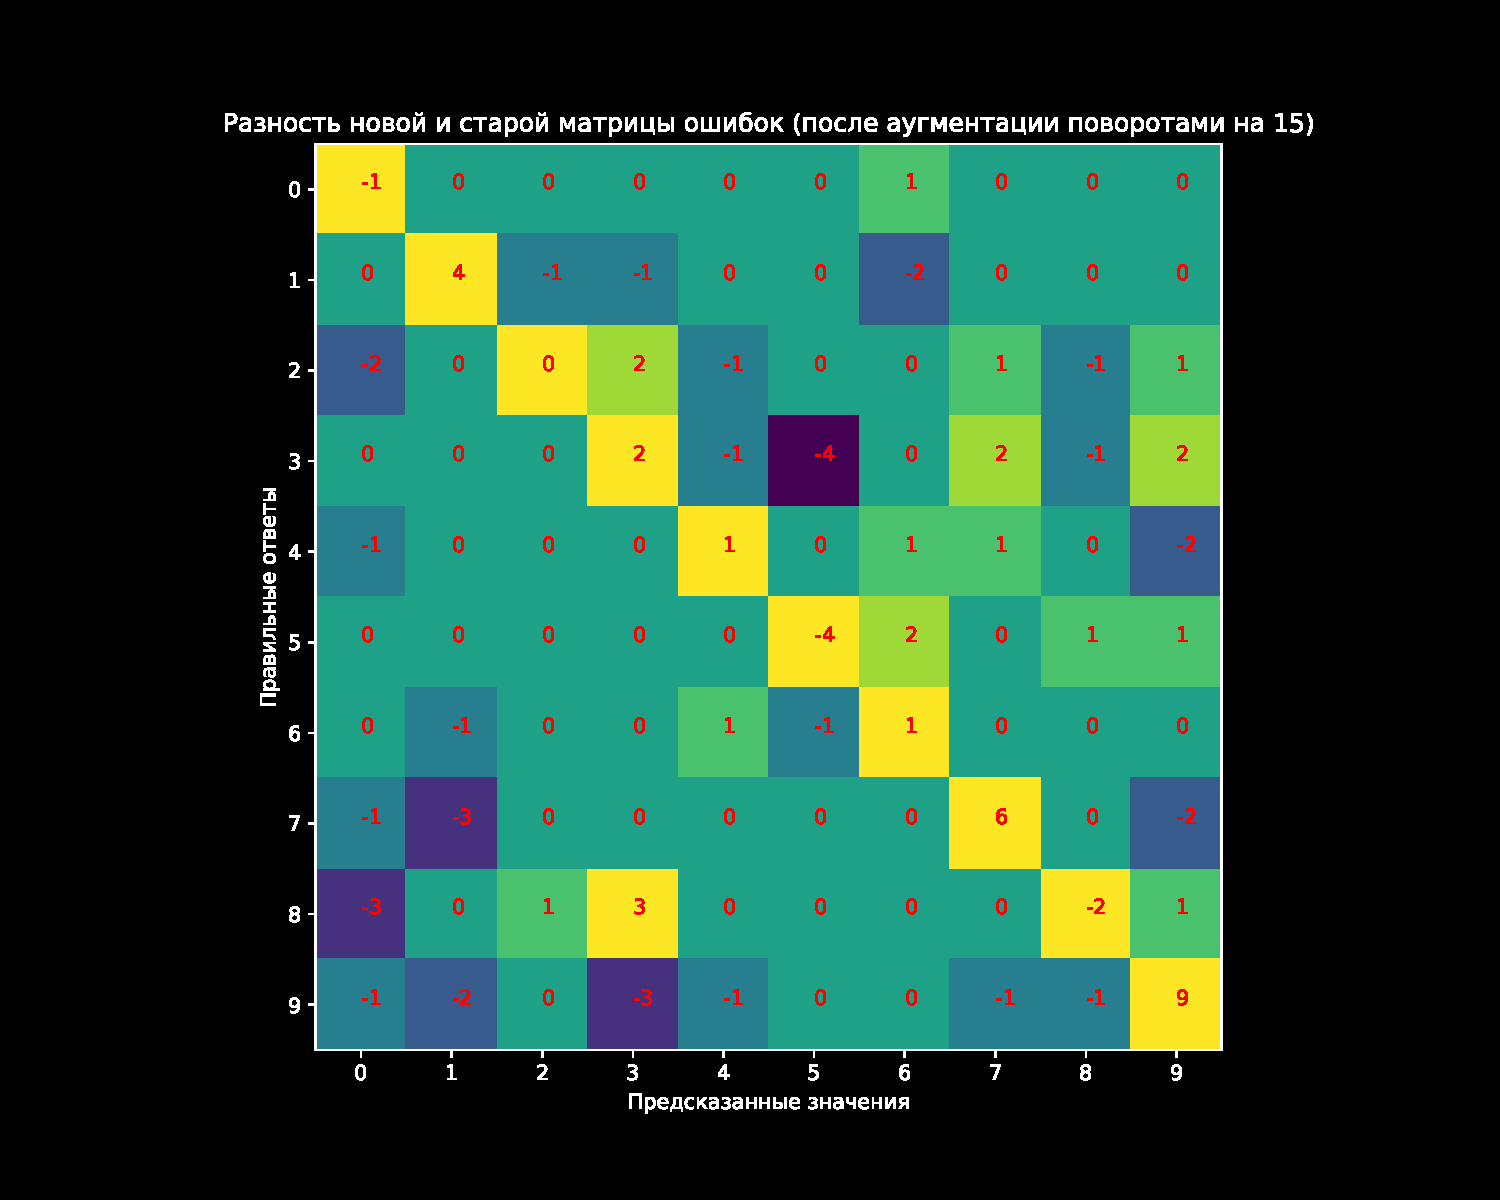
\includegraphics[width=0.8\linewidth]{./pictures/ConfusionDifferenceRotate5.pdf}
            \caption{Динамика ошибок при применении поворотов}
            \label{fig:mpr}
        \end{figure}
        \begin{figure}[H]
            \centering
            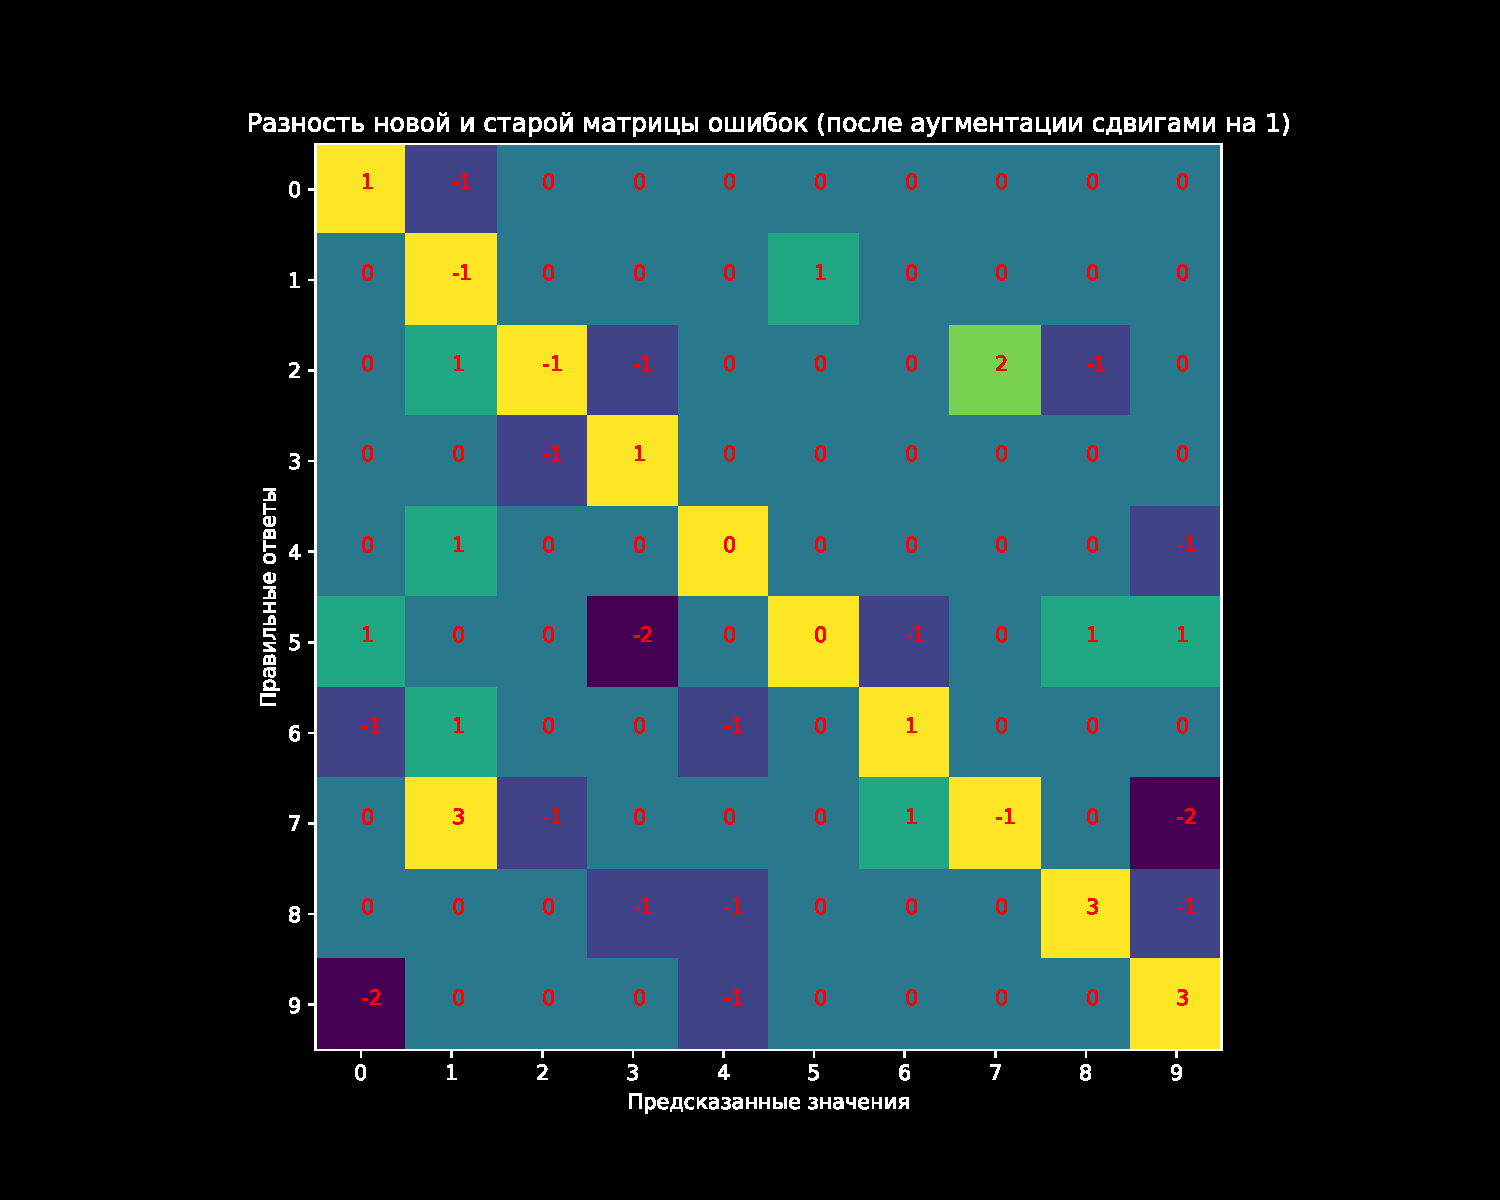
\includegraphics[width=0.8\linewidth]{./pictures/ConfusionDifferenceShift5.pdf}
            \caption{Динамика ошибок при применении сдвига}
            \label{fig:mpr}
        \end{figure}
        \begin{figure}[H]
            \centering
            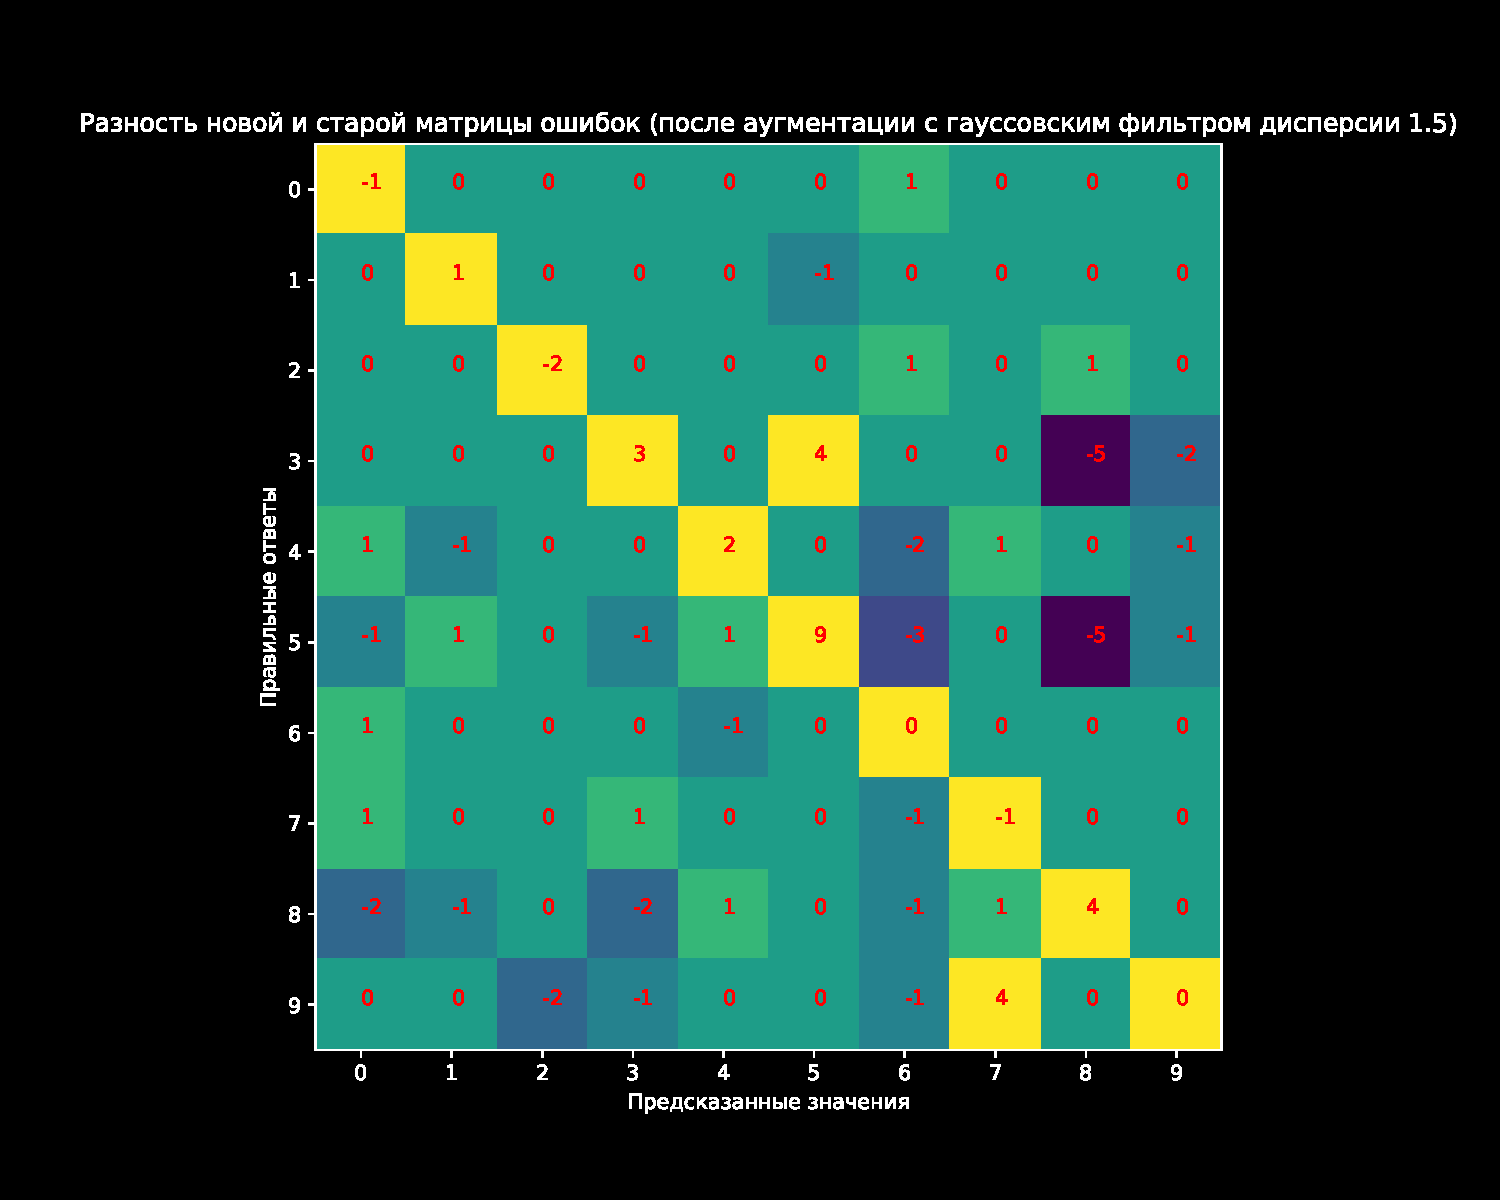
\includegraphics[width=0.8\linewidth]{./pictures/ConfusionDifferenceBlur5.pdf}
            \caption{Динамика ошибок при применении гауссова фильтра}
            \label{fig:mpr}
        \end{figure}
        \begin{figure}[H]
            \centering
            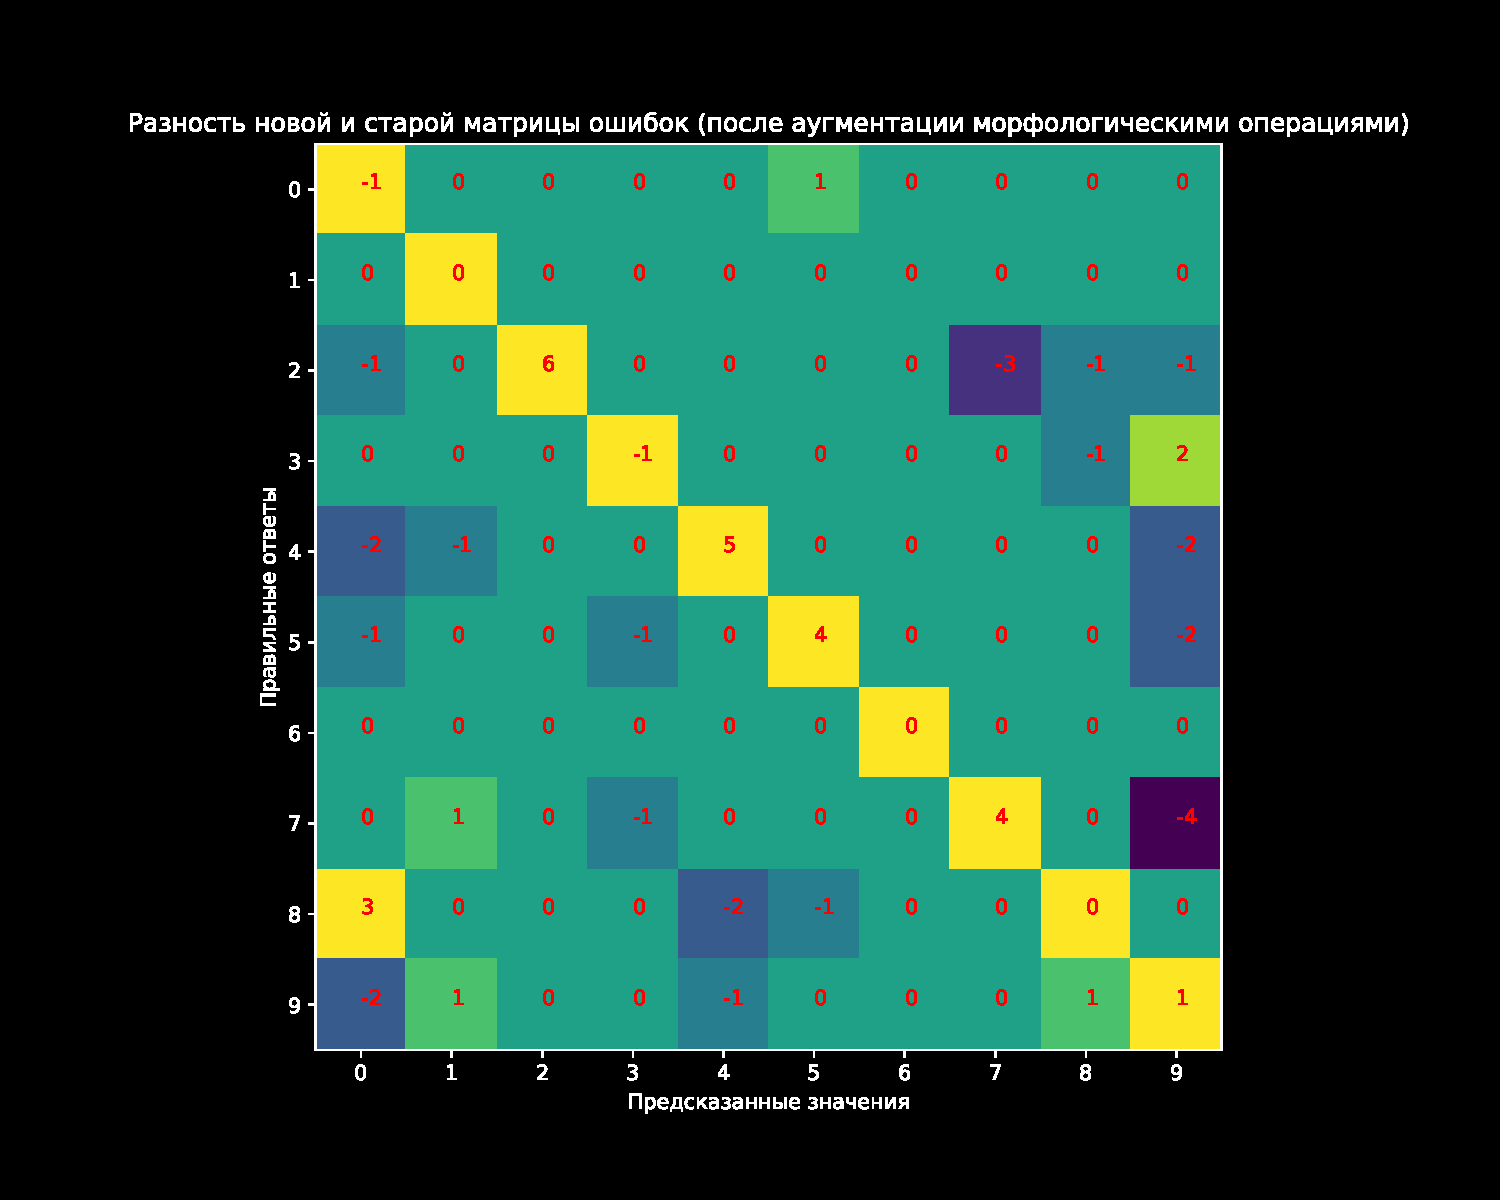
\includegraphics[width=0.8\linewidth]{./pictures/ConfusionDifferenceMorph5.pdf}
            \caption{Динамика ошибок при применении эрозии, дилации, открытия и закрытия}
            \label{fig:mpr}
        \end{figure}
\end{document}
